% INavigationPolicy lifecycle across a volume traversal (Gen3).
% Call sites in Core/src/Navigation/Navigator.cpp as annotated.
% Note: isValid() defaults to `true` in INavigationPolicy.hpp:265-271 and NO concrete
% policy in Core overrides it - so Gen3 never re-resolves inside a volume.
\documentclass[border=8pt]{standalone}
\usepackage{tikz}
\usepackage{newtxtext,newtxmath}
\usetikzlibrary{arrows.meta,positioning,calc,decorations.pathreplacing,backgrounds}

\begin{document}
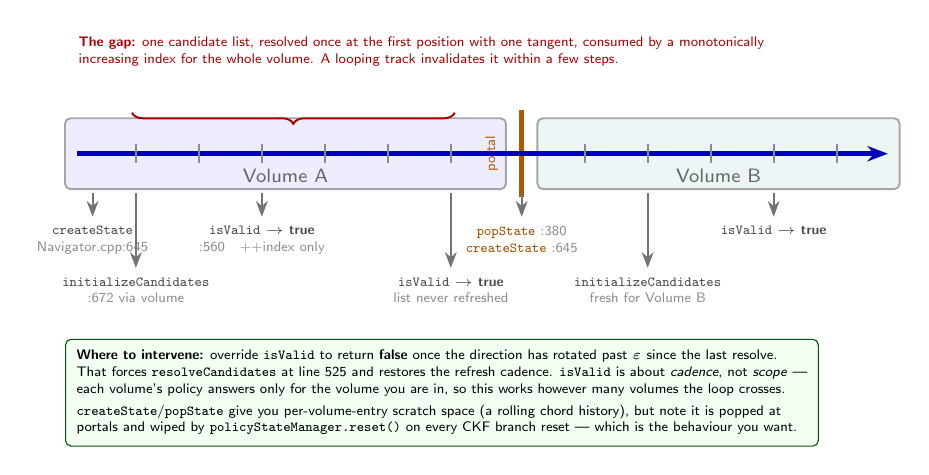
\begin{tikzpicture}[
  scale=1.0,
  font=\sffamily\footnotesize,
  vol/.style={draw=black!35,rounded corners=2pt,line width=0.7pt},
  ev/.style={-{Stealth[length=2.0mm]},line width=0.7pt,draw=black!55},
  lbl/.style={font=\sffamily\scriptsize},
  tny/.style={font=\sffamily\tiny},
  tick/.style={line width=0.6pt,draw=black!45}
]

% ---- volume bands ----
\fill[blue!7,rounded corners=2pt]  (0,1.55) rectangle (5.6,2.45);
\fill[teal!7,rounded corners=2pt]  (6.0,1.55) rectangle (10.6,2.45);
\draw[vol] (0,1.55) rectangle (5.6,2.45);
\draw[vol] (6.0,1.55) rectangle (10.6,2.45);
\node[lbl,text=black!60] at (2.8,1.72) {Volume A};
\node[lbl,text=black!60] at (8.3,1.72) {Volume B};

% portal
\draw[line width=1.6pt,draw=orange!70!black] (5.8,1.45) -- (5.8,2.55);
\node[tny,text=orange!70!black,rotate=90,anchor=south] at (5.62,2.0) {portal};

% ---- trajectory ----
\draw[line width=1.6pt,draw=blue!72!black,-{Stealth[length=2.6mm]}]
  (0.15,2.0) -- (10.45,2.0);

% ---- step ticks ----
\foreach \x in {0.9,1.7,2.5,3.3,4.1,4.9,6.6,7.4,8.2,9.0,9.8} {
  \draw[tick] (\x,1.88) -- (\x,2.12);
}

% ---- events below ----
\newcommand{\evt}[4]{%
  \draw[ev] (#1,1.50) -- (#1,#2);
  \node[tny,anchor=north,align=center,text=#4] at (#1,#2) {#3};
}

\evt{0.35}{1.20}{\texttt{createState}\\ \textcolor{black!45}{Navigator.cpp:645}}{black!70}
\evt{0.9}{0.55}{\texttt{initializeCandidates}\\ \textcolor{black!45}{:672 via volume}}{black!70}
\evt{2.5}{1.20}{\texttt{isValid} $\rightarrow$ \textbf{true}\\ \textcolor{black!45}{:560 \ \ ++index only}}{black!70}
\evt{4.9}{0.55}{\texttt{isValid} $\rightarrow$ \textbf{true}\\ \textcolor{black!45}{list never refreshed}}{black!70}
\evt{5.8}{1.20}{\texttt{popState} \textcolor{black!45}{:380}\\ \texttt{createState} \textcolor{black!45}{:645}}{orange!65!black}
\evt{7.4}{0.55}{\texttt{initializeCandidates}\\ \textcolor{black!45}{fresh for Volume B}}{black!70}
\evt{9.0}{1.20}{\texttt{isValid} $\rightarrow$ \textbf{true}}{black!70}

% ---- the gap ----
\draw[decorate,decoration={brace,amplitude=4pt},draw=red!65!black,line width=0.7pt]
  (4.95,2.52) -- (0.85,2.52);
\node[tny,text=red!65!black,anchor=south,align=center] at (2.9,2.60)
  {};
\node[tny,text=red!65!black,anchor=west,align=left] at (0.05,3.30)
  {\textbf{The gap:} one candidate list, resolved once at the first position with one tangent,
   consumed by a monotonically\\
   increasing index for the whole volume. A looping track invalidates it within a few steps.};

% ---- the hook ----
\node[draw=green!35!black,fill=green!5,rounded corners=2pt,inner sep=4pt,
      align=left,tny,anchor=north west] at (0.0,-0.35)
  {\textbf{Where to intervene:} override \texttt{isValid} to return \textbf{false} once the direction has
   rotated past $\varepsilon$ since the last resolve.\\
   That forces \texttt{resolveCandidates} at line 525 and restores the refresh cadence.
   \texttt{isValid} is about \emph{cadence}, not \emph{scope} ---\\
   each volume's policy answers only for the volume you are in, so this works however many volumes
   the loop crosses.\\[2pt]
   \texttt{createState}/\texttt{popState} give you per-volume-entry scratch space (a rolling chord history),
   but note it is popped at\\
   portals and wiped by \texttt{policyStateManager.reset()} on every CKF branch reset ---
   which is the behaviour you want.};

\end{tikzpicture}
\end{document}
